\documentclass{beamer}
\usetheme{Madrid}
\usepackage{amsmath, amssymb, amsthm}
\usepackage{graphicx}
\usepackage{listings}
\usepackage{gensymb}
\usepackage[utf8]{inputenc}
\usepackage{hyperref}
\usepackage{gvv}
\usepackage{tikz}
\lstset{
  language=Python,
  basicstyle=\ttfamily\small,
  keywordstyle=\color{blue},
  stringstyle=\color{orange},
  numbers=left,
  numberstyle=\tiny\color{gray},
  breaklines=true,
  showstringspaces=false
}
\usetikzlibrary{decorations.pathmorphing}

\title{Question-3.0.22}
\author{EE25BTECH11022 - sankeerthan}
\date{}
\begin{document}

\frame{\titlepage}
% Slide 1: Problem
\begin{frame}{Problem Statement}
Let $X_1, X_2, \dots, X_5$ be a random sample of size $5$ from a population of having standard normal distribution $N\brak{0,1}$.Let
\begin{align}
\bar{X} = \frac{1}{5}\sum_{i=1}^{5} X_i
\\
T = \sum_{i=1}^{5} \brak{X_i - \bar{X}}^2.
\end{align}
Find
\begin{align}
E\brak{T^2 \bar{X}^2}.
\end{align}

\end{frame}


\begin{frame}{Solution}
\begin{itemize}
\item $\bar{X}$ measures the  $\brak{mean}$
\item $T$ measures the $\brak{variance}$
\item In normal distribution, these are independent
\end{itemize}
\begin{align}
\Rightarrow E\brak{T^2 \bar{X}^2} = E\brak{T^2}\,E\brak{\bar{X}^2}
\end{align}
\end{frame}


\begin{frame}{Properties of $X_i$}
Given: \\
\begin{align}
 X_i \sim N\brak{0,1}
\end{align}
\\
\textbf{Compare With} 
\begin{align}
N\brak{\mu, \sigma^2} \Rightarrow \mu =\text{mean},\sigma^2 = \text{variance}
\end{align}\\
\begin{itemize}
\item Mean = 0
\item Variance = 1
\end{itemize}
\end{frame}

\begin{frame}{Mean of $\bar{X}$}
\begin{align}
\bar{X} &= \frac{1}{5}\brak{X_1 + X_2 + \cdots + X_5}\\
E\brak{\bar{X}} &= \frac{1}{5}\brak{E\brak{X_1}+\cdots+E\brak{X_5}}\\
&= \frac{1}{5}\brak{0+0+0+0+0} \\
&= 0
\end{align}
\end{frame}

\begin{frame}{Variance of $\bar{X}$}
\begin{align}
\text{Var}\brak{X_1 + \cdots + X_5} &= 1+1+1+1+1 = 5\\
\bar{X} &= \frac{1}{5}\brak{X_1 + \cdots + X_5}\\
\text{Var}\brak{\bar{X}} &= \text{Var}\brak{\frac{1}{5}\brak{X_1 + \cdots + X_5}} \\
 &=\frac{1}{25} \times 5 \\
 &= \frac{1}{5}
\\
\end{align}
\textbf{As We Know That}
\begin{itemize}
\item Variance adds for independent variables
\item $\text{Var}\brak{cX} = c^2 \text{Var}\brak{X}$
\end{itemize}
\end{frame}

\begin{frame}{Finding $E\brak{\bar{X}^2}$}
\begin{align}
E\brak{\bar{X}} &= 0 \\
\text{Var}\brak{\bar{X}} &= E\brak{\bar{X}^2} - \sbrak{E\brak{\bar{X}}}^2 \\
\frac{1}{5} &= E\brak{\bar{X}^2} - 0   \\
E\brak{\bar{X}^2} &= \frac{1}{5}
\end{align}
\end{frame}

% Slide 7: Understanding T
\begin{frame}{Understanding $T$ using Chi-Square Distribution}
\begin{align}
T &= \sum \brak{X_i - \bar{X}}^2 \\
&= \sum X_i -5\bar{X}^2 \\
&T \sim \chi^2_{n-1}\\
&T \sim\chi^2_4
\end{align}
\textbf{Reason:}
If $T= \sum X_i$ ,then $T \sim \chi^2_i$ .
But here instead of $X_i$, $\brak{X_i-\bar{X}}$ is present .
So,One degree of freedom is lost due to $\bar{X}$
\end{frame}

% Slide 8: Mean and Variance of T
\begin{frame}{Properties of $T$ and Finding $E\brak{T^2}$}
For $\chi^2_k$:
\begin{align}
E\brak{T} &= k = 4  \\
\text{Var}\brak{T} &= 2k = 8 \\
\text{Var}\brak{T} &= E\brak{T^2} - \sbrak{E\brak{T}}^2 \\
E\brak{T^2} &= \text{Var}\brak{T} + \sbrak{E\brak{T}}^2 \\
&= 8 + 16 \\
&= 24
\end{align}
\end{frame}

\begin{frame}{Final Calculation}
\begin{align}
E\brak{T^2 \bar{X}^2} &= E\brak{T^2}\,E\brak{\bar{X}^2}\\
&= 24 \times \frac{1}{5} \\
&= \frac{24}{5} \\
\end{align}
\end{frame}

\begin{frame}{Conclusion}
\textbf{Method Summary:}
\begin{itemize}
\item Use independence of $\bar{X}$ and $T$
\item Find $E\brak{\bar{X}^2}$ using variance
\item Use chi-square properties for $T$
\item Multiply results
\end{itemize}
\textbf{Final Answer:}
\begin{align}
E\brak{T^2 \bar{X}^2} =\frac{24}{5}
\end{align}
\end{frame}
\begin{frame}
\frametitle{graph}
\begin{figure}
    \centering
    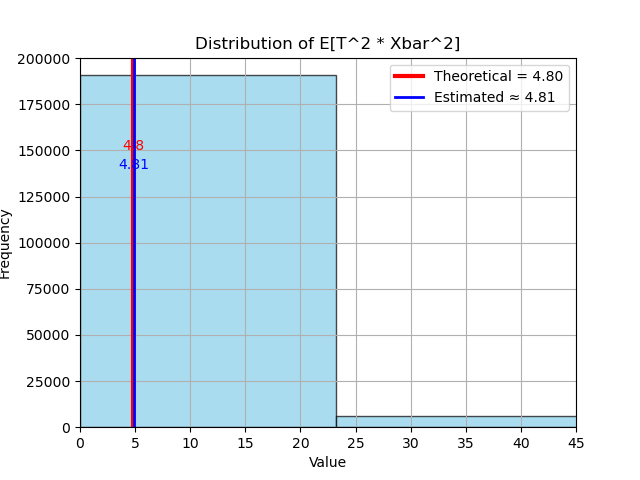
\includegraphics[width=0.7\columnwidth]{figs/Figure_1.png}
    \caption{}
\end{figure}
\end{frame}
\begin{frame}[fragile]
\frametitle{Python-Code}
\begin{lstlisting}
import numpy as np
import matplotlib.pyplot as plt

samples = 200000
values = np.zeros(samples)

# Simulation
for s in range(samples):
    X = np.random.normal(0, 1, 5)
    Xbar = np.mean(X)
    T = np.sum((X - Xbar)**2)
    values[s] = (T**2) * (Xbar**2)

estimated_value = np.mean(values)
theoretical_value = 24 / 5

print("Estimated =", estimated_value)
print("Theoretical =", theoretical_value)
\end{lstlisting}
\end{frame}
\begin{frame}[fragile]
\frametitle{Python-Code}
\begin{lstlisting}
plt.figure()

# Histogram
plt.hist(values, bins=30, color='skyblue', edgecolor='black', alpha=0.7)

#  Slight shift for visibility
offset = 0.1

# Theoretical line (red)
plt.axvline(theoretical_value, color='red', linestyle='--', linewidth=3,
            label=f'Theoretical = {theoretical_value:.2f}')

# Estimated line (blue, slightly shifted)
plt.axvline(estimated_value + offset, color='blue', linestyle='-', linewidth=2,
            label=f'Estimated ≈ {estimated_value:.2f}')
\end{lstlisting}
\end{frame}
\begin{frame}[fragile]
\frametitle{Python-Code}
\begin{lstlisting}
#  Add text labels near lines
plt.text(theoretical_value, 150000, "4.8", color='red', ha='center')
plt.text(estimated_value + offset, 140000, f"{estimated_value:.2f}", color='blue', ha='center')

# Better scaling
plt.xlim(0, 45)
plt.ylim(0, None)

plt.title("Distribution of E[T^2 * Xbar^2]")
plt.xlabel("Value")
plt.ylabel("Frequency")
plt.legend()
plt.grid()
plt.show()
\end{lstlisting}
\end{frame}

\end{document}